\esSezione{Multiplexer 16:1}\label{sec:esercizio1-1}

\begin{traccia}
Progettare, implementare in VHDL e testare mediante simulazione un multiplexer indirizzabile 16:1, utilizzando un approccio di progettazione per composizione a partire da multiplexer 4:1.
\end{traccia}

\progetto

Realizziamo il multiplexer 16:1 con un'architettura modulare ad albero, ovvero attraverso due livelli di multiplexer 4:1. Al primo livello troviamo quattro componenti: ognuno riceve un gruppo di quattro ingressi consecutivi e i due bit meno significativi della selezione. Le loro uscite alimentano un quinto multiplexer 4:1, pilotato dai due bit più significativi della selezione, e l'uscita di quest'ultimo è quella del top module. Il top module ha quindi venti ingressi complessivi, sedici dati e quattro di selezione, e un'unica uscita. Lo schema è visibile in figura~\ref{fig:esercizio1-1:schema}.

\begin{figure}[H]
  \centering
  \begin{tikzpicture}[node distance=1cm]
    % primo livello
    \node[blocco, minimum width=2.2cm] (m0) at (0,0)    {\texttt{M0}\\mux\_4\_1};
    \node[blocco, minimum width=2.2cm] (m1) at (0,-2.8) {\texttt{M1}\\mux\_4\_1};
    \node[blocco, minimum width=2.2cm] (m2) at (0,-5.6) {\texttt{M2}\\mux\_4\_1};
    \node[blocco, minimum width=2.2cm] (m3) at (0,-8.4) {\texttt{M3}\\mux\_4\_1};
    % secondo livello
    \node[blocco, minimum width=2.2cm, minimum height=2.4cm] (m4) at (6.2,-4.2) {\texttt{M4}\\mux\_4\_1};
    % ingressi dati
    \foreach \n in {m0,m1,m2,m3}
      \draw[bus] ($(\n.west)+(-1.9,0)$) -- node[pos=0.65, sloped, inner sep=1pt]{/} node[pos=0.65, above=3pt, font=\scriptsize]{4} (\n.west);
    \node[font=\scriptsize\ttfamily, anchor=east] at ($(m0.west)+(-1.9,0)$) {a(0 to 3)};
    \node[font=\scriptsize\ttfamily, anchor=east] at ($(m1.west)+(-1.9,0)$) {a(4 to 7)};
    \node[font=\scriptsize\ttfamily, anchor=east] at ($(m2.west)+(-1.9,0)$) {a(8 to 11)};
    \node[font=\scriptsize\ttfamily, anchor=east] at ($(m3.west)+(-1.9,0)$) {a(12 to 15)};
    % selezione primo livello
    \foreach \n in {m0,m1,m2,m3}
      \draw[bus] ($(\n.south)+(0,-1.4)$) -- node[pos=0.35, sloped, inner sep=1pt]{/} node[pos=0.35, left=3pt, font=\scriptsize]{2} (\n.south);
    \foreach \n in {m0,m1,m2,m3}
      \node[font=\scriptsize\ttfamily, anchor=west] at ($(\n.south)+(0.15,-0.9)$) {s(1 downto 0)};
    % uscite primo livello: bus u
    \draw[seg] (m0.east) -| ($(m4.west)+(-0.4,0.9)$) -- ($(m4.west)+(0,0.9)$);
    \draw[seg] (m1.east) -| ($(m4.west)+(-0.8,0.3)$) -- ($(m4.west)+(0,0.3)$);
    \draw[seg] (m2.east) -| ($(m4.west)+(-0.8,-0.3)$) -- ($(m4.west)+(0,-0.3)$);
    \draw[seg] (m3.east) -| ($(m4.west)+(-0.4,-0.9)$) -- ($(m4.west)+(0,-0.9)$);
    \node[font=\scriptsize\ttfamily, anchor=south] at ($(m0.east)+(1.0,0)$) {u(0)};
    \node[font=\scriptsize\ttfamily, anchor=south] at ($(m1.east)+(1.0,0)$) {u(1)};
    \node[font=\scriptsize\ttfamily, anchor=south] at ($(m2.east)+(1.0,0)$) {u(2)};
    \node[font=\scriptsize\ttfamily, anchor=south] at ($(m3.east)+(1.0,0)$) {u(3)};
    % selezione secondo livello e uscita
    \draw[bus] ($(m4.south)+(0,-1.4)$) -- node[pos=0.35, sloped, inner sep=1pt]{/} node[pos=0.35, left=3pt, font=\scriptsize]{2} (m4.south);
    \node[font=\scriptsize\ttfamily, anchor=west] at ($(m4.south)+(0.15,-0.9)$) {s(3 downto 2)};
    \draw[seg] (m4.east) -- ++(1.2,0) node[right, font=\scriptsize\ttfamily] {y};
  \end{tikzpicture}
  \caption{MUX 16:1}
  \label{fig:esercizio1-1:schema}
\end{figure}

Nello schema \texttt{u} indica il segnale interno di quattro bit che raccoglie le uscite del primo livello e ne costituisce il vettore di ingresso per \texttt{M4}.

\implementazione

Partiamo dal componente elementare, l'entità \texttt{mux\_4\_1}, che ha come porte \texttt{a}, vettore di quattro ingressi dati indicizzato da 0 a 3, \texttt{s}, selezione a due bit, e \texttt{y}, uscita a un bit. L'architettura \texttt{dataflow} usa un'assegnazione \texttt{with select}: a ogni valore di \texttt{s} corrisponde un ingresso, mentre per i valori non validi l'uscita assume \texttt{'-'}. 

\vhdlfile{esercizio1-1/mux_4_1.vhd}{Implementazione MUX 4:1}{lst:esercizio1-1:mux-4-1}

Definito tale componente, vediamo il top module \texttt{mux\_16\_1}, che ha come porte il vettore \texttt{a} di sedici ingressi (indici da 0 a 15), la selezione \texttt{s} a quattro bit e l'uscita \texttt{y}. L'architettura è \texttt{structural}: il segnale interno \texttt{u}, di quattro bit, raccoglie le uscite dei componenti \texttt{M0}, \texttt{M1}, \texttt{M2} ed \texttt{M3}, istanziati con port mapping sui gruppi \texttt{a(0 to 3)}, \texttt{a(4 to 7)}, \texttt{a(8 to 11)} e \texttt{a(12 to 15)} e con \texttt{s(1 downto 0)} come selezione. Il componente \texttt{M4} riceve \texttt{u} come vettore di ingressi, ha \texttt{s(3 downto 2)} come selezione e produce \texttt{y}. 

\vhdlfile{esercizio1-1/mux_16_1.vhd}{Implementazione MUX 16:1}{lst:esercizio1-1:mux-16-1}

\simulazione

Il testbench \texttt{mux\_16\_1\_tb} ha un'entità priva di porte, poiché non deve essere istanziato. Contiene un'istanza del top module con port mapping sui segnali \texttt{i} (sedici bit, indici da 0 a 15), \texttt{s} (quattro bit) e \texttt{y}. Il process \texttt{stimuli} attende \SI{100}{ns}, assegna a \texttt{i} il valore \texttt{"0010110101001010"} e poi percorre con un ciclo \texttt{for} i valori di \texttt{j} da 0 a 15: a ogni iterazione pone \texttt{s} pari a \texttt{j} (conversione con \texttt{to\_unsigned}), attende \SI{10}{ns} e verifica con un \texttt{assert} che \texttt{y} coincida con \texttt{i(j)}; in caso contrario la simulazione termina con \texttt{severity failure}. Il \texttt{wait} finale sospende il process. Si riporta di seguito il testbench.

\vhdlfile{esercizio1-1/mux_16_1_tb.vhd}{Testbench MUX 16:1}{lst:esercizio1-1:mux-16-1-tb}

La figura~\ref{fig:esercizio1-1:simulazione} mostra il risultato della simulazione. L'ingresso \texttt{i} resta costante al valore 0x2D4A ($0010\,1101\,0100\,1010_2$), mentre la selezione \texttt{s} assume in successione i valori da 0x0 a 0xF con un passo di \SI{10}{ns}, a partire da \SI{100}{ns}.

\begin{figure}[H]
  \centering
  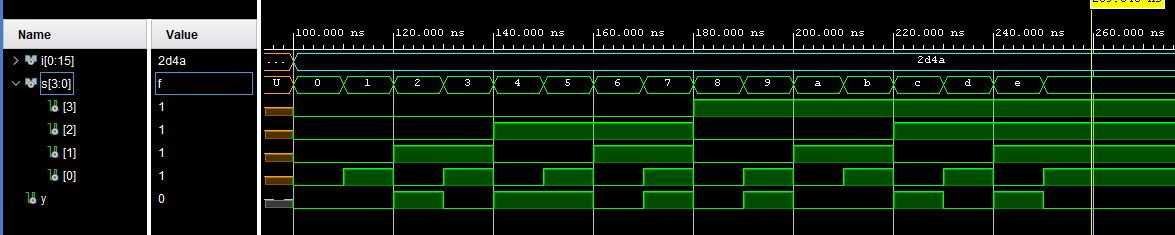
\includegraphics[width=0.95\linewidth]{figure/esercizio1-1/simulazione}
  \caption{Simulazione MUX 16:1}
  \label{fig:esercizio1-1:simulazione}
\end{figure}

